\documentclass[12pt]{article}
\usepackage{graphicx}
\usepackage{subcaption}
\usepackage{hyperref}
\usepackage{float}

\title{CMSC 6950 Project}
\date{June 2021}
\author{Yashar Tavakoli} 

\setlength\parindent{0pt}
\begin{document}
\maketitle
\section{Introduction}

This project in a nutshell, aims at fetching data from \verb|argopy|, manipulating the data a bit, and presenting the results
through proper visualization. \verb|argopy| landing page states that it aims to 
\begin{enumerate}
    \item ease argo data access, 
    \item manipulation, and
    \item visualization. 
\end{enumerate} 
In my experience, visualization facilities of the argo is quite limited. So I have employed more powerful python
libraries for visualization. Without further without further adieu, I will explain the two computational tasks I
took on.

\section{Density of argos' locations}

Every argo during its lifetime visits sequence of 
locations (at different depth). Having said that, the frequency of
locations (in form longitude and latitude pairs) within every geographical boundary over a certain period of time,
would be non-uniform. So an interesting question would be: in given a geographical boundary in the form of a box defined
by latitude and longitude coordinates, which points are visited by argos and how much?\\

Scatter-plot would be a quick approach to this problem. Scatter-plots however suffer from certain shortcomings:

\begin{itemize}
    \item When the data is dense, a scatter plot would be messy less interpret-able to the eye. 
    \item There is no visual component accompanying scatter-plots, whereby one can learn the exact number of points in a given region.
\end{itemize}

A workaround in this situation would be some sort of 2-dimensional \textit{destiny plot}, whereby
the distribution of data is more readily observable. \\

One of the more sophisticated density plots perhaps, is 
\verb|seaborn.kdeplot|. 
But seaborn is not integrated with \verb|mpl_toolkits.basemap|,
which is the library I will use for the underlay geographical 
map (a map-less plot would also suffer from poor interpret-ability). 
Instead of \verb|seaborn.kdeplot|, I will use 
\verb|matplotlib.pyplot.hexbin| which
is well integrated with \verb|basemap|.\\

Now regarding the geographically bounded argo data, 
during a given time period:
 \begin{itemize}
     \item One can use \verb|argo_loader.region().to_xarray()| which takes longitude, latitude, and time period as arguments, and 
     returns the argo data in multidimensional \verb|xarray|.
     \item Since working
     with Pandas (2-dimensional) data-frames is more straightforward, 
     I have flattened the \verb|xarrays| 
     (using \verb|argo.point2profile()|),
     and converted them to Panda's data-frames 
     (using \verb|to_dataframe()|).
     \item Flattening a multidimensional \verb|xarray| to 
     2-dimensional produces a multi-index data-frame. 
     In computation task no.1, 
     we do not need any of the indices so I have discarded 
     the indices (using \verb|reset_index()|). Furthermore I 
     have dismissed all
     the columns but longitude and latitude. 
     Lastly before 
     drawing the \verb|matplotlib.pyplot.hexbin| on the map, I have
     prepared the data for \verb|mpl_toolkits.basemap|.
 \end{itemize}

 As depicted Fig.\ref{hexbin} in The region I have chosen for 
 this task stretches from 140 to 150 
 in longitude, and from 35 to 50 in latitude (around Japan). 
 The time-frame is chosen to be a six months period between 
 2015-06-01 and 2015-12-30. The image depicts the result. One
 last step I performed is highlighting some locations on the map 
 to be able to better explain the plot: It seems to be
 more-or-less to say that argos cover offshore more frequently 
 than ports such as Sendai. One exception perhaps, would be
 off the coast of Sapporo (in Hokkaido) with more than 1000 profile 
 reports. One curious fact is argos' low frequency north of Kunashiri.    

\begin{figure}[!htb]
\centering
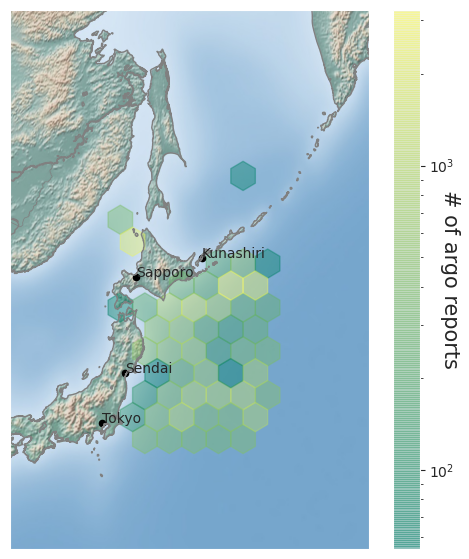
\includegraphics[scale=0.9]{hexbin_argos_locations.png}
\caption{Hexbin plot of argo data}
\label{hexbin}
\end{figure}

\section{A correlation analysis of Level, Pressure, Salinity, 
and Temperature.}

A question one might ask regarding argo data, would be the correlation 
between each pair in Level, 
Pressure, Salinity, and Temperature. To keep the computations light, 
I have singled out four profiles from four different
argos located in Indian Ocean, South Atlantic, North Atlantic, and 
Pacific (using the service provided by 
\href{https://fleetmonitoring.euro-argo.eu/dashboard?Status=Active}{fleetmonitoring.euro-argo}). Now to fetch  
the data I have used \verb|argo_loader.profile().to_xarray()|, which 
takes the argo WMO and profile numbers, and returns the data
in the form of four different \verb|xarrays| (I have chosen profile 
numbers 
manually, so that the produced plots show decent diversity).\\

Next, as explained in task no.1, I have flattened the \verb|xarrays| 
and converted them to Panda's data-frames. Here, unlike
task no.1, the produced indices in the data-frames are not useless: 
the Level variable the data-frames is defined as 
index. As a first step, I have reintroduced Level as a column and 
dismissed all the column except Level, Pressure, 
Salinity, and Temperature.\\

Before moving forward, let's take a look at a map produced by 
\verb|basemap| hinting at the spots where
the chosen argos resided or have resided (Fig.\ref{map}). 
Since each profile consists of a sequence of longitudes and 
latitudes,
I have taken a mean to get an idea about the whereabouts of 
the argos pertaining to the selected profiles.\\

Now back to the main task at hand, we need a proper 
visualization which help us get an idea of the correlation
between the variables in question. To do this I have 
devised a composite plot from thee components: 

\begin{enumerate}
    \item The lower-triangle consists of pairwise scatter-plots.
    \item The diagonal consists of histogram bars illustrating 
    the distribution of variables.
    \item The upper-triangle indicates the Pearson's r 
    coefficient for each pair of variables 
    (implemented though \verb|reg_coef()| 
    in the code). The Pearson's r ranges from 1 to -1.
    A value close to 1 (-1) indicates a (reverse) near
    perfect linear relationship between the variables.
    A value close to 0, implies that there is almost no 
    linear correlation between the variables.
\end{enumerate}



Now lets take a couple of notes regarding the
correlation between the variables as illustrated in
Fig.\ref{corr}:
    
\begin{itemize}
    \item The scatter plots and coefficients for all the cases 
    indicate a near-perfectly
    linear relationship between Pressure and Level. 
    \item All the plots also demonstrate that there exist a 
    significant reverse linear relationship between Temperature 
    and Level,
    as well as Temperature and Pressure.
    \item The rest of the pair of variables show non-conclusive 
    behavior. The situation here would entail a more educated 
    investigation. That said, curiously there is no near-zero 
    coefficient for any of the pairs.
    \item The variables are similarly correlated pertaining to 
    profiles from Indian Ocean, South Atlantic. Same with North Atlantic
    and North Pacific. So a crude non-educated guess: the divide 
    is between northern and southern hemisphere??
\end{itemize}


\begin{figure}[!htb]
    \centering
    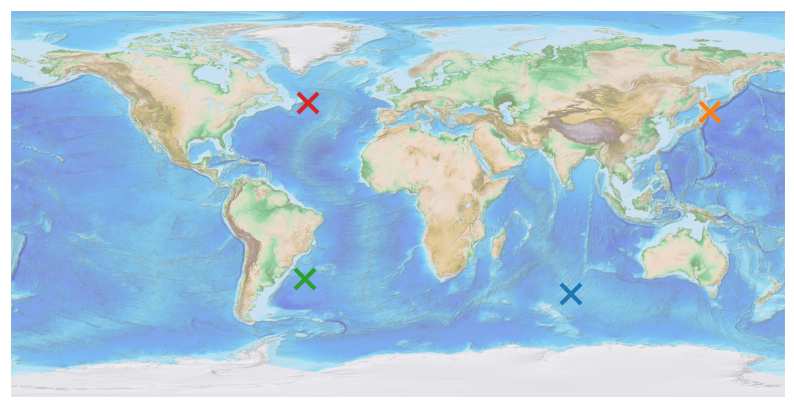
\includegraphics[scale=0.7]{map_of_locations.png}
    \caption{Locations of the argos}
    \label{map}
\end{figure}
    
    
\begin{figure}[!htb]
\begin{tabular}{cc}
    \hspace{-30pt} 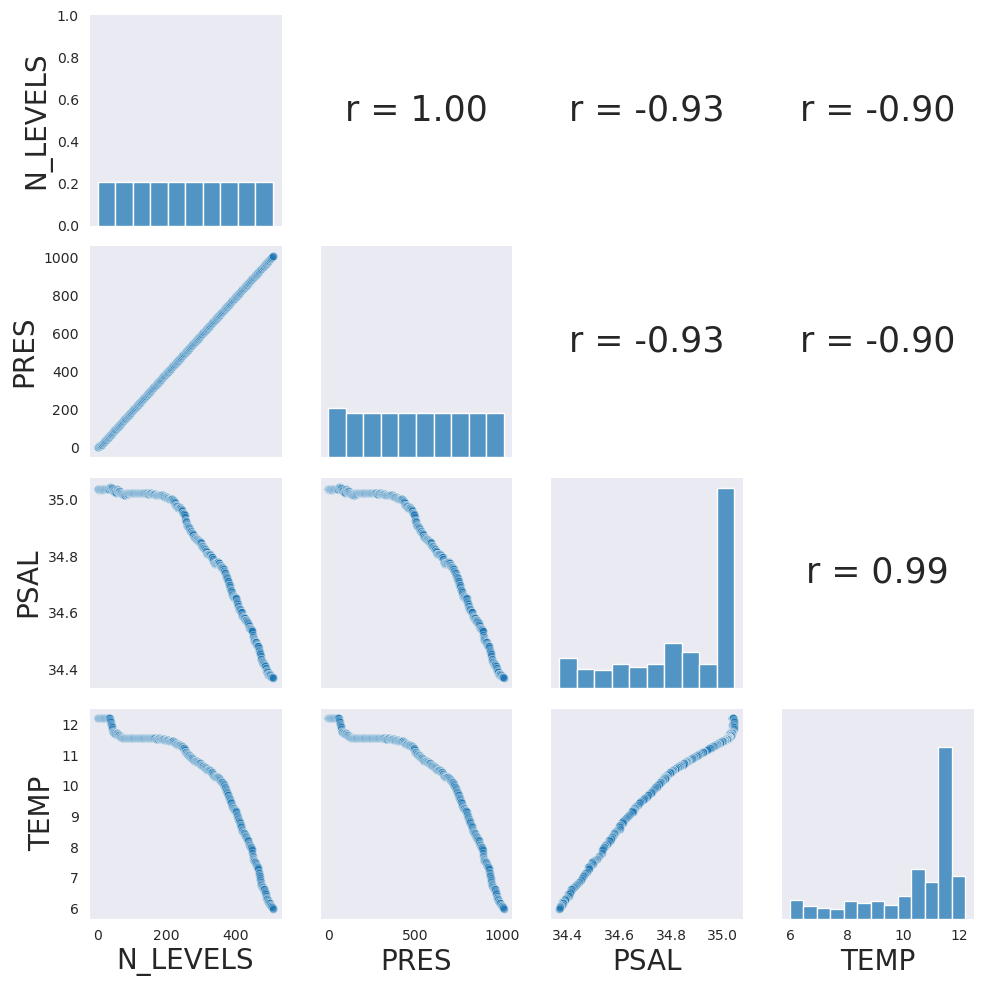
\includegraphics[width=70mm]{correlation1.png} &\hspace{10pt}   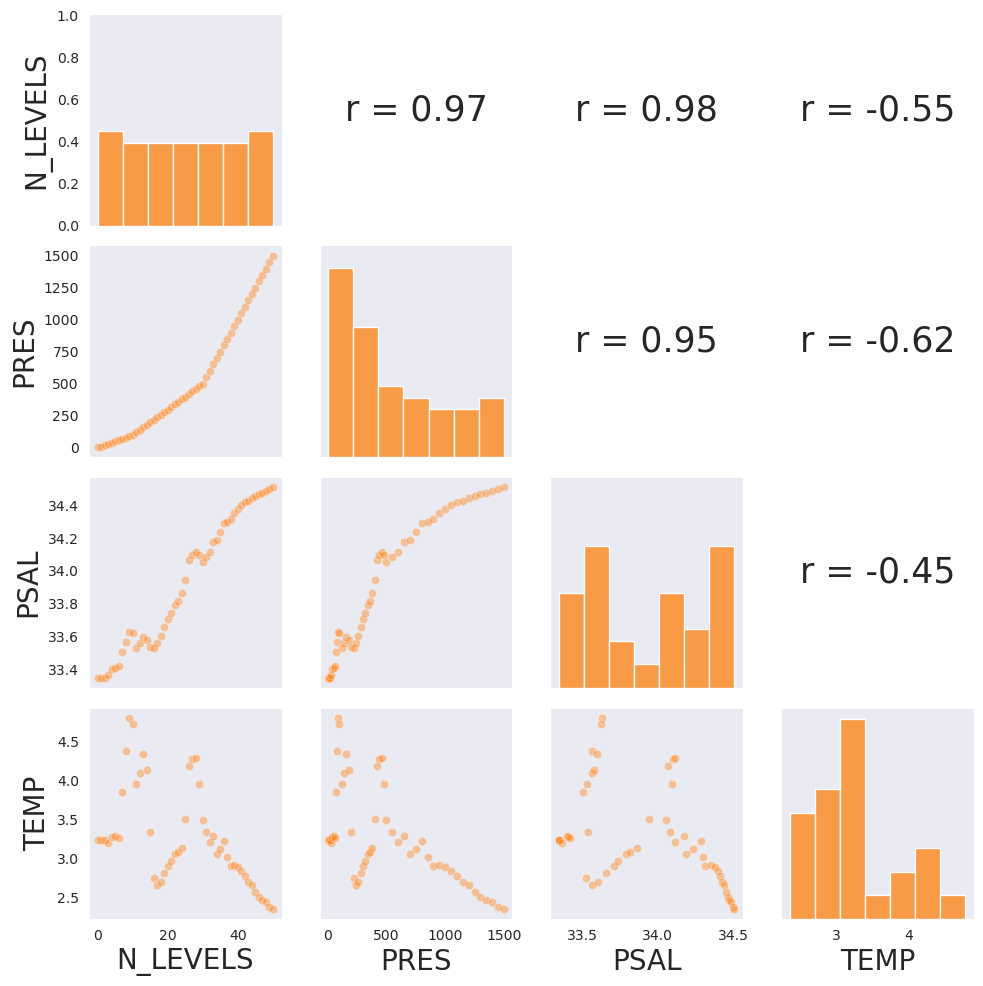
\includegraphics[width=70mm]{correlation2.png} \\
    (a) Location: Indian Ocean & (b) Location: North Pacific \\[15pt]
    \hspace{-30pt} 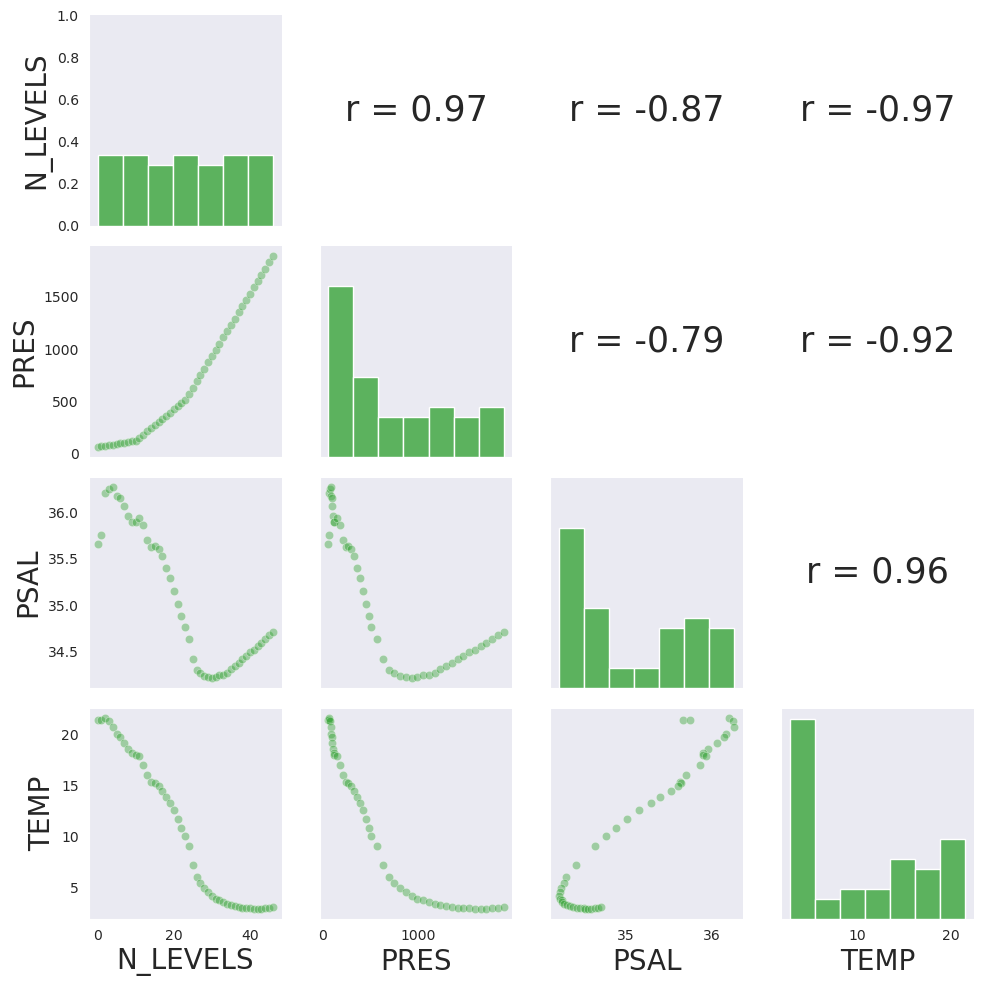
\includegraphics[width=70mm]{correlation3.png} &\hspace{10pt}   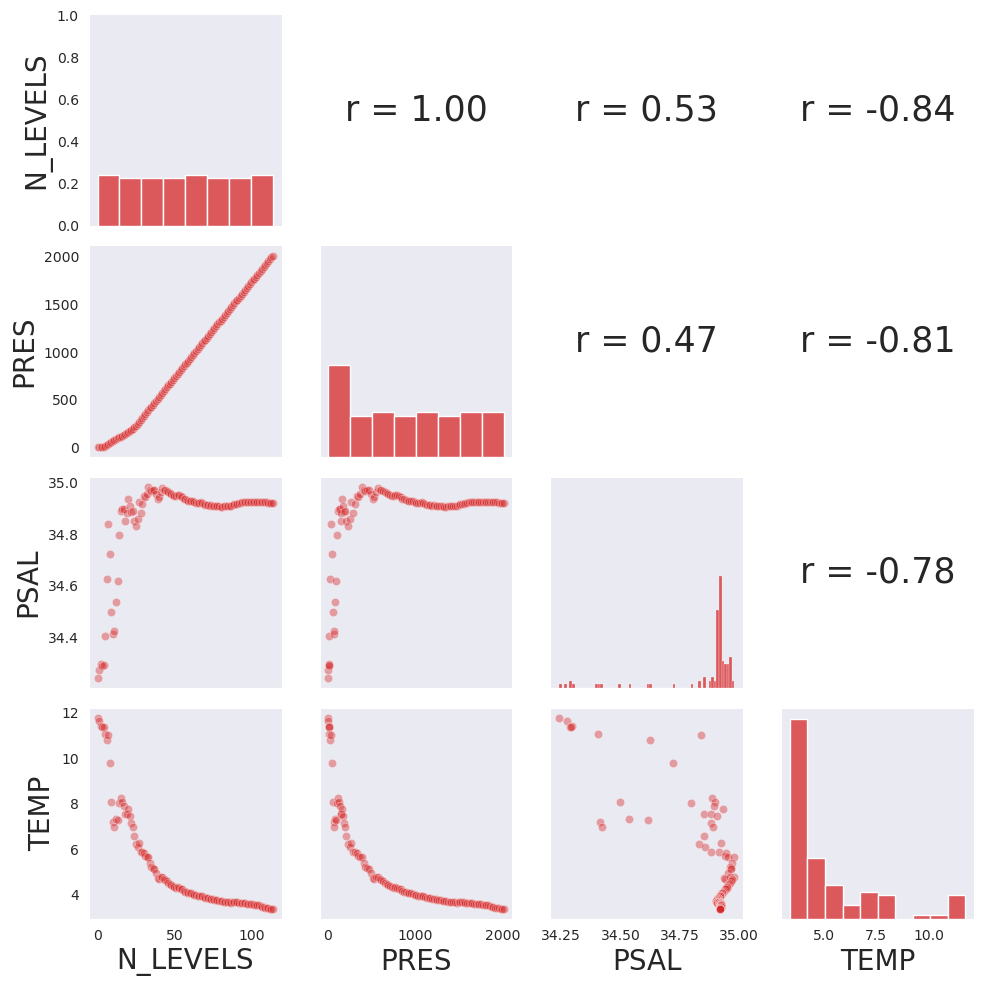
\includegraphics[width=70mm]{correlation4.png} \\
    (c) Location: South Atlantic & (d) Location: North Atlantic \\[15pt]
    \end{tabular}
    \caption{Correlation between the variables}
    \label{corr}
\end{figure}

\begin{thebibliography}{9}
    \bibitem{latexcompanion} 
    Maze et al.,
    \textit{argopy: A Python library for Argo ocean data analysis.}. 
    Journal of Open Source Software, 5(53), 2425, 2020.
\end{thebibliography}

\end{document}